\documentclass[12pt]{scrartcl}

 
\usepackage{float}
\usepackage[utf8]{inputenc}

\usepackage[T1]{fontenc}

\usepackage{lmodern}

\usepackage[ngerman]{babel}

\usepackage{amsmath}

\usepackage{graphicx}


 

\title{Versuch AK1\\ Ultraschall}

\author{Frederik Strothmann, Henrik Jürgens}

\date{\today}


\begin{document}


 %deckblatt erstellen

\maketitle
\newpage
\tableofcontents
\newpage

%einleitung zu dem experiment

\section{Einleitung}
Mit einem System aus piezoelektrischen Ultraschallsendern und -empfängern wird die Schallgeschwindigkeit in Luft
bestimmt nach der Phasen- und der Laufzeitmethode. Bei Kenntnis der Schallgeschwindigkeit kann die Laufzeitmethode zur Entfernungsmessung eingesetzt werden (Echolotprinzip). Eine Anordnung mit zwei gleichen Ultraschallsendern wirkt wie ein Doppelspalt und liefert ein typisches
Ultraschall-Interferenzmuster, das ausgemessen werden soll.
Außerdem sollen noch die elektrischen Eigenschaften des Piezosenders (Impedanz) untersucht werden.

%versuchsaufbau mit skizze

\section{Versuchsaufbau}
Für diesen Versuch werden ein Oszilloskop, ein Funktionsgenerator, eine optische Bank mit zwei Reitern zur Montage des Ultraschallsenders und Empfängers (inklusive Strahlhörner), sowie ein Doppelsender verwendet. Für die einzelnen Versuchsteile werden zusätzlich ein elektronischer Unterbrecher, sowie ein Kasten zur Impedanzmessung benötigt (siehe Abbildung \ref{fig:impedanz}). Die genauen Aufbauten sind in den praktischen Durchführungen des jeweiligen Aufgabenteils zu finden.

\begin{figure}[htbp] 
  \centering
    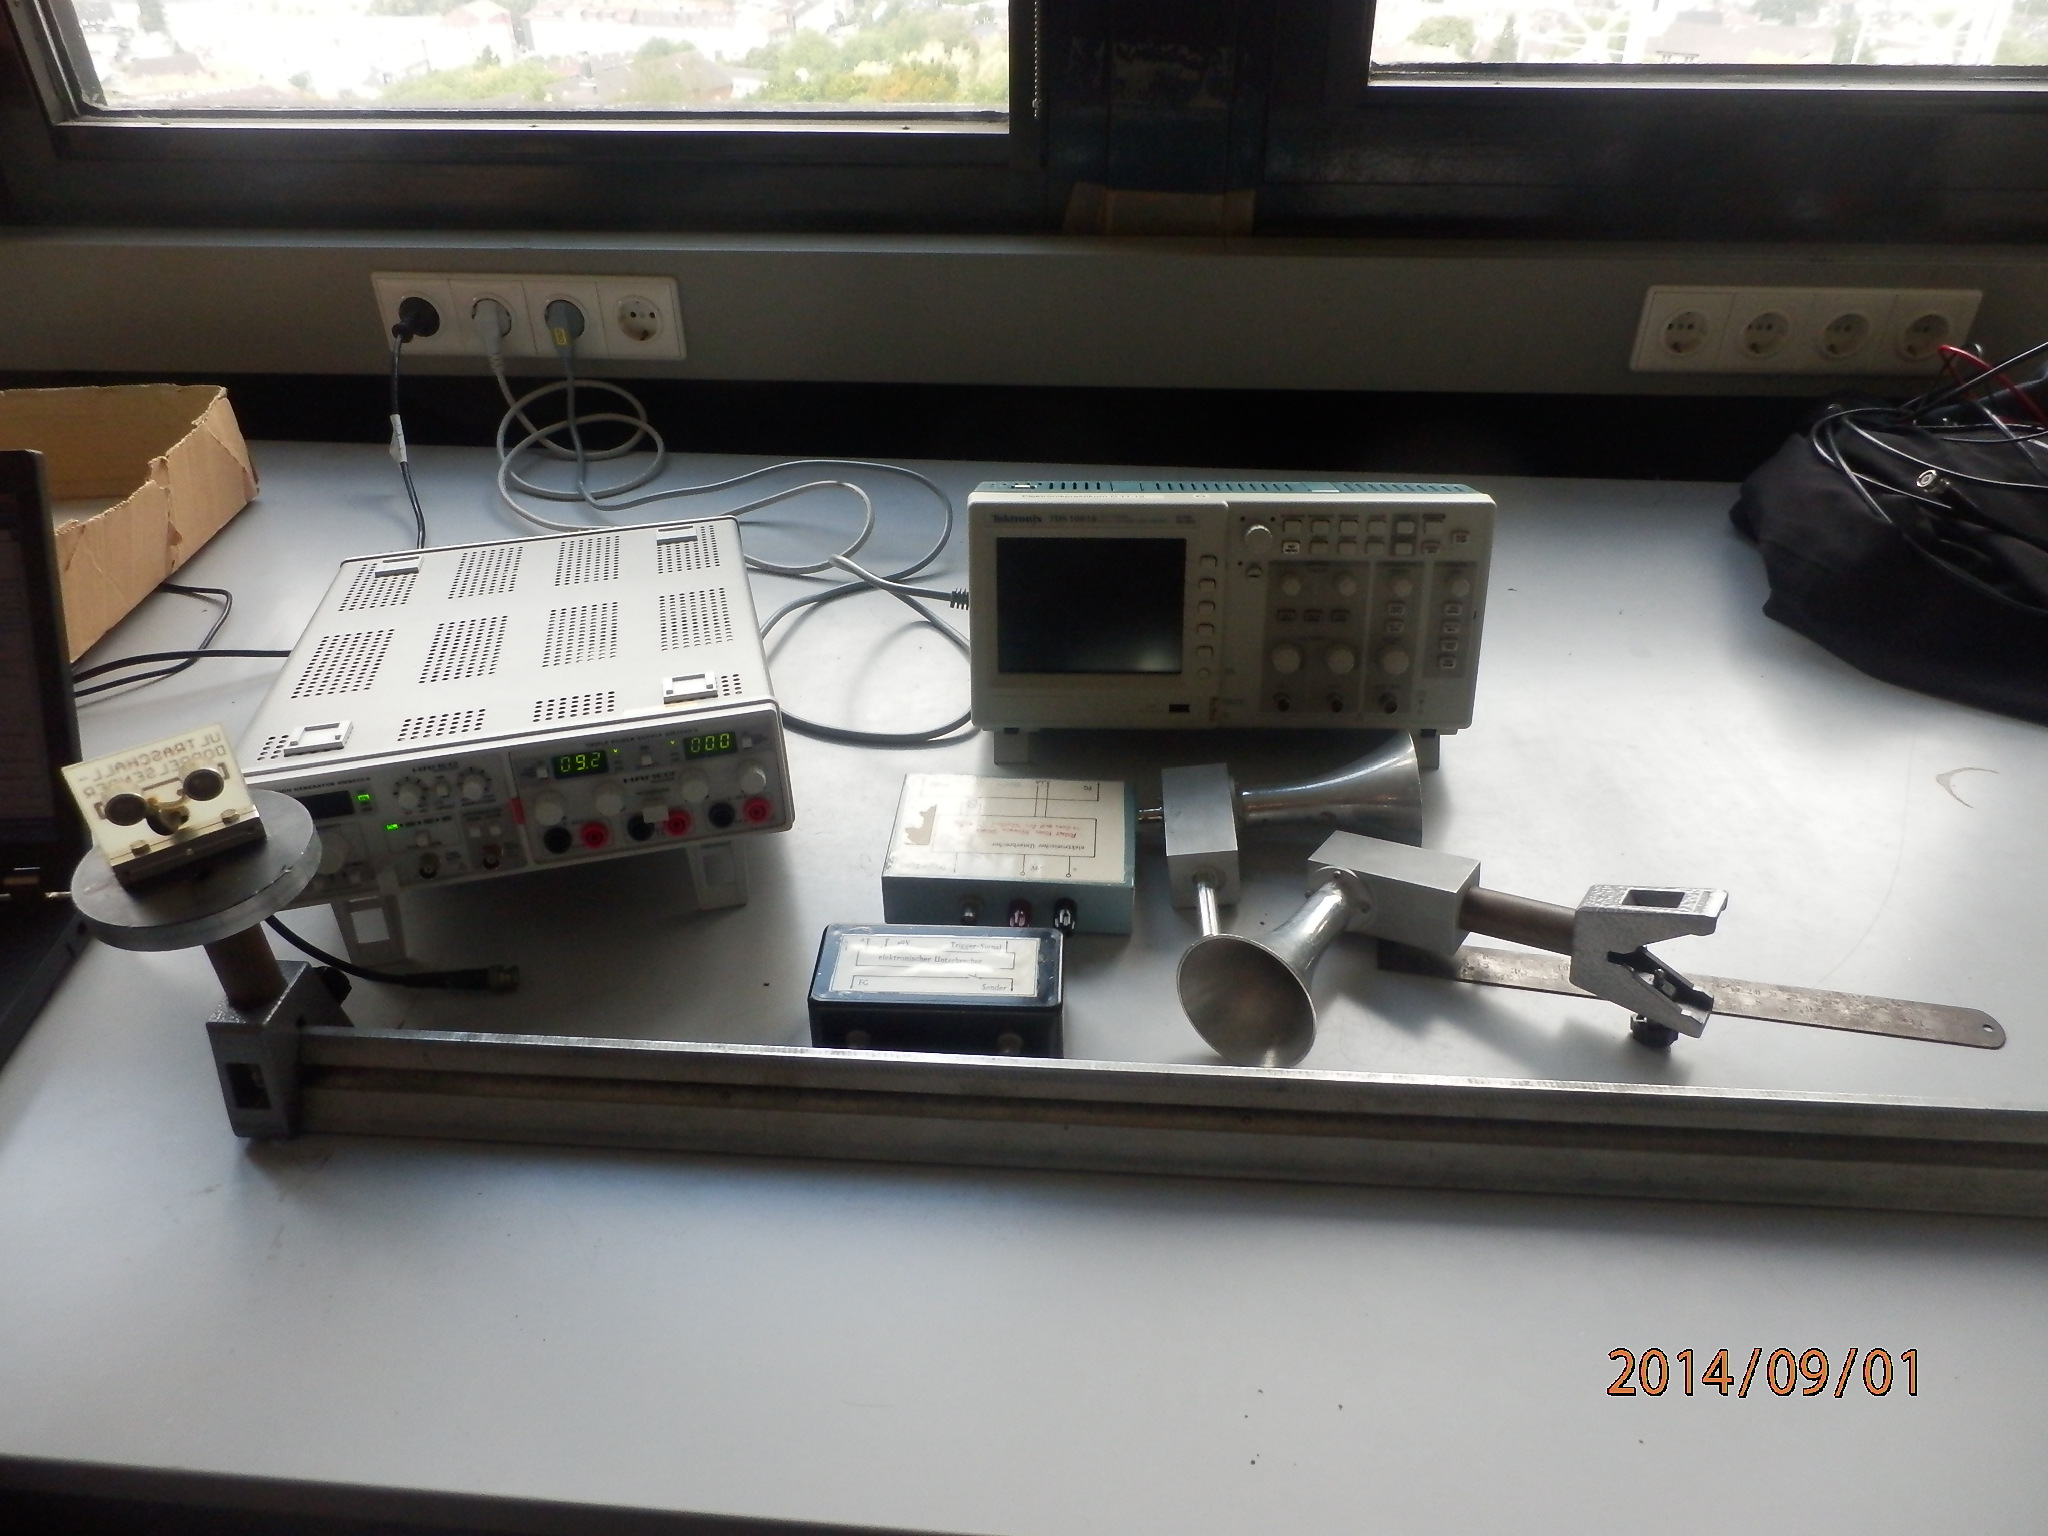
\includegraphics[scale = 0.1]{versuchsaufbau.JPG}
  	\caption[Abbildung der Verwendeten Gerätschaften]{Abbildung der Verwendeten Gerätschaften}
  \label{fig:impedanz}
\end{figure}


\section{Aufgabe 1 Impedanzmessung}
\subsection{Versuchsdurchführung}
\subsubsection{Praktische Durchführung}
\begin{itemize}
\item[(a)]
Um die elektrischen Eigenschaften eines Barium-Titanat-Ultraschallgenerators zu untersuchen, wird eine Schaltung gemäß Abb. \ref{fig:impedanz}
aufgebaut. Stellen Sie am Funktionsgenerator ein Sinussignal mit einer Amplitude von etwa 5 V ein.
%bitte Abb.7 aus der Versuchsanleitung einfügen, welche grade referenziert werden sollte "Aufbau zur Impedanzmessung"
\begin{figure}[htbp] 
  \centering
    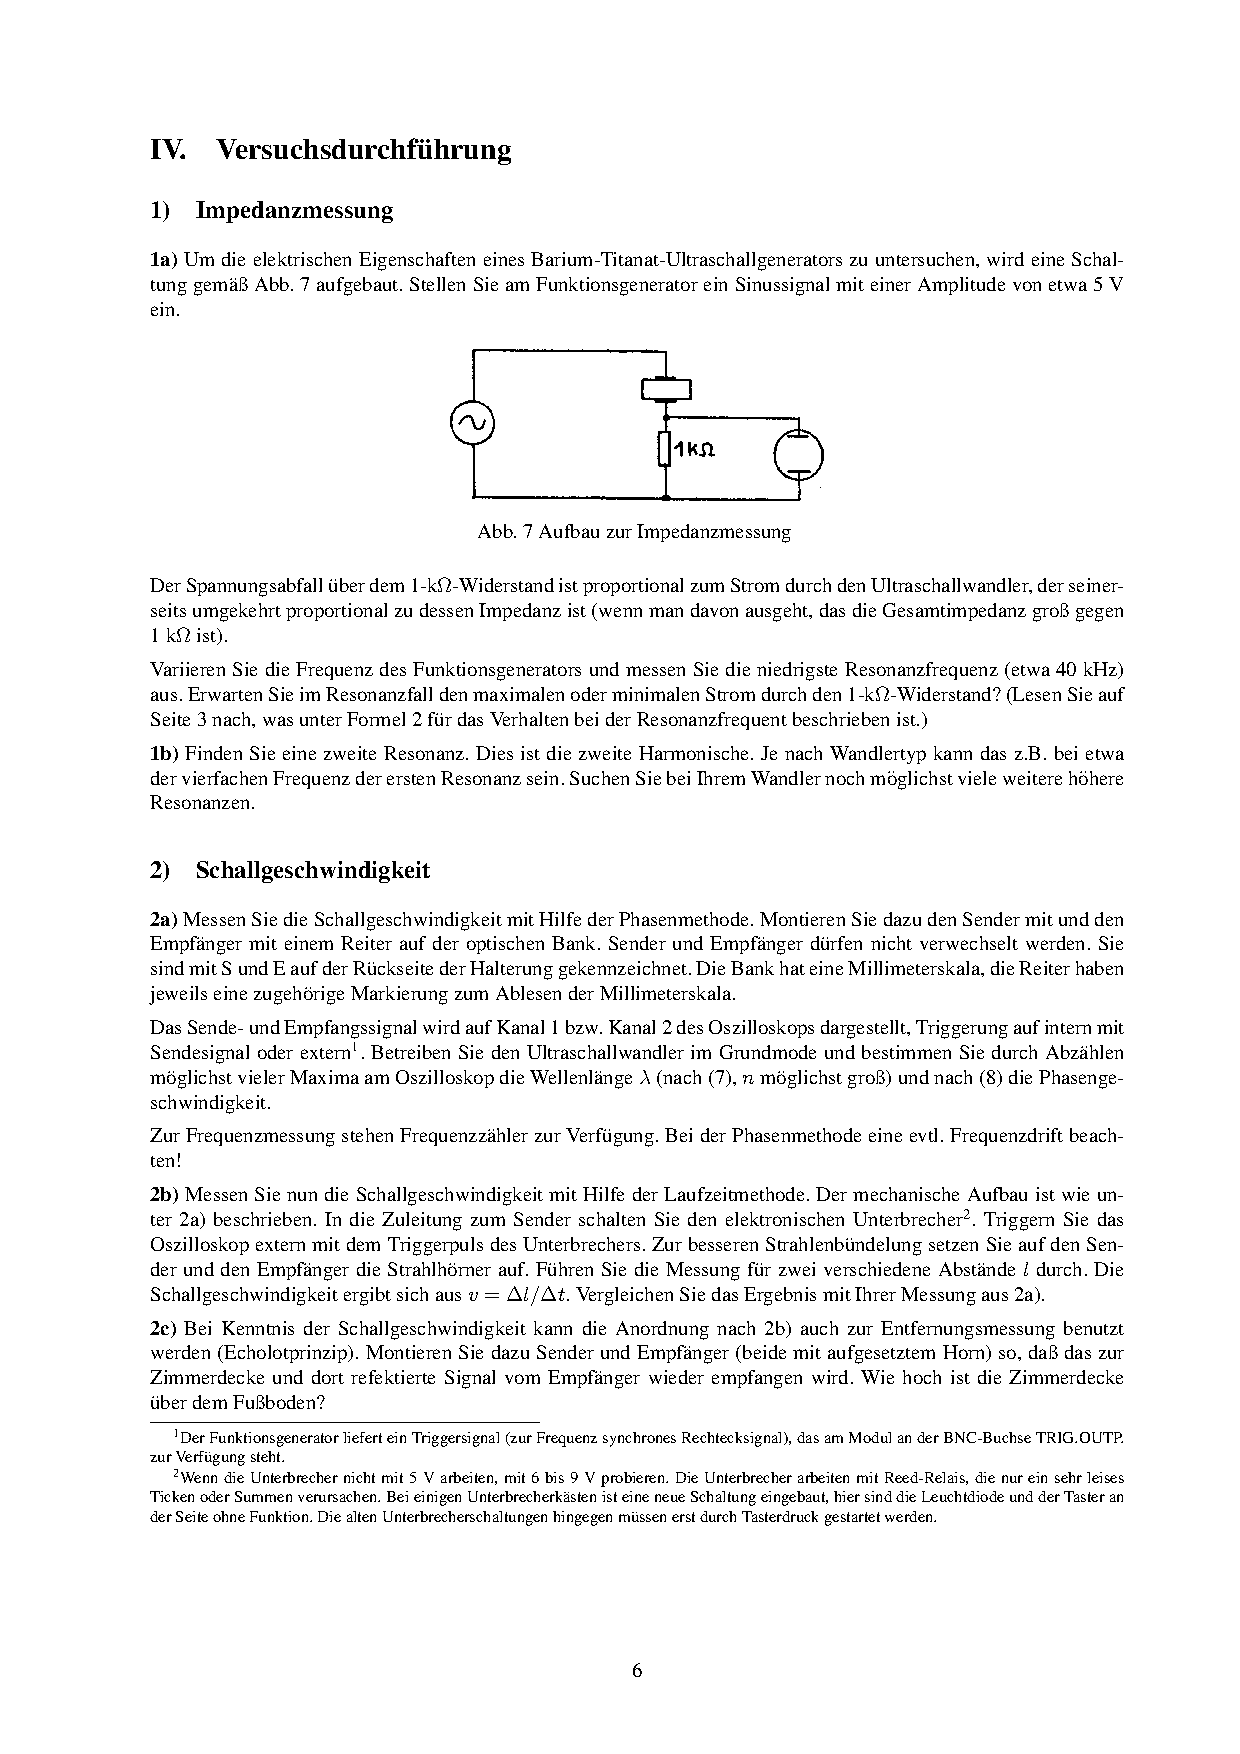
\includegraphics[trim = 20mm 210mm 20mm 55mm, clip, scale = 1]{impedanz.pdf}
  	\caption[Schaltskizze des Versuchsaufbaus]{Schaltskizze des Versuchsaufbaus\footnotemark}
  \label{fig:impedanz}
\end{figure}
\footnotetext{Abbildung entnommen von http://www.atlas.uni-wuppertal.de/~kind/AK1.pdf Seite 6 am 30.08.2014}
Der Spannungsabfall über dem 1-k$\Omega$-Widerstand ist proportional zum Strom durch den Ultraschallwandler, der seinerseits umgekehrt proportional zu dessen Impedanz ist (wenn man davon ausgeht, das die Gesamtimpedanz groß gegen 1 k$\Omega$ ist).
Variieren Sie die Frequenz des Funktionsgenerators und messen Sie die niedrigste Resonanzfrequenz (etwa 40 kHz)
aus. Erwarten Sie im Resonanzfall den maximalen oder minimalen Strom durch den 1-k$\Omega$-Widerstand? 
%(Lesen Sie auf Seite 3 nach, was unter Formel 2 für das Verhalten bei der Resonanzfrequenz beschrieben ist.)
\item[(b)]
Finden Sie eine zweite Resonanz. Dies ist die zweite Harmonische. Je nach Wandlertyp kann das z.B. bei etwa der vierfachen Frequenz der ersten Resonanz sein. Suchen Sie bei Ihrem Wandler noch möglichst viele weitere höhere
Resonanzen.
\end{itemize}
\subsection{Messergebnisse}
\begin{table}[H]
\caption{Die gemessenen Resonanzfrequenzen}
\begin{center}
\begin{tabular}{|r|}
\hline
Resonanzfrequenz/Hz \\ \hline
41750$(\pm 500)$ \\ \hline
53660$(\pm 500)$ \\ \hline
162900$(\pm 1000)$ \\ \hline
249700$(\pm 1000)$ \\ \hline
604000$(\pm 1000)$ \\ \hline
\end{tabular}
\end{center}
\label{tab:aufgabe1}
\end{table}
\subsection{Auswertung}
Im ersten Teil von Aufgabe 1 sollte die erste Resonanzfrequenz bestimmt und ausgemessen werden. Dabei ergab sich ein Wert von 41750$(\pm 500)$Hz. Danach sollten weitere Resonanzfrequenzen bestimmt werden, wobei sich die folgenden Frequenzen  aus den Messdaten (Tabelle \ref{tab:aufgabe1}) ergaben, 53660$(\pm 500)$Hz, 162900$(\pm 1000)$Hz, 249700$(\pm 1000)$Hz und 604000$(\pm 1000)$Hz.
\subsection{Diskussion}
Die gemessenen Resonanzfrequenzen waren zum Teil sehr schwierig zu messen, da das Minimum oft nicht eindeutig bestimmt werden konnte.
Wir mussten bei höheren Frequenzen, bedingt durch die größere Ableseungenauigkeit am Frequenzgenerator und nur noch schwach ausgeprägten Minima, größe Fehler annehmen.
Bei 53660 Hz wurde gegen die Erwartungen ein Minimum gemessen, was wir uns nicht direkt erklären konnten. Vermutlich hatten anderen Materialien, die für unseren Aufbau verwendet wurden bzw. im Sender befestigt waren einfluss auf unsere Messung. 
\section{Aufgabe 2 Schallgeschwindigkeit}
\subsection{Versuchsdurchführung}
\subsubsection{Praktische Durchführung}
\begin{itemize}
\item[(a)]
Messen Sie die Schallgeschwindigkeit mit Hilfe der Phasenmethode. Montieren Sie dazu den Sender mit und den Empfänger mit einem Reiter auf der optischen Bank. Sender und Empfänger dürfen nicht verwechselt werden. Sie sind mit S und E auf der Rückseite der Halterung gekennzeichnet. Die Bank hat eine Millimeterskala, die Reiter haben
jeweils eine zugehörige Markierung zum Ablesen der Millimeterskala. Das Sende- und Empfangssignal wird auf Kanal 1 bzw. Kanal 2 des Oszilloskops dargestellt, Triggerung auf intern mit Sendesignal oder extern
\footnote{Der Funktionsgenerator liefert ein Triggersignal (zur Frequenz synchrones Rechtecksignal), das am Modul an der BNC-Buchse TRIG.OUTP. zur Verfügung steht.}. Betreiben Sie den Ultraschallwandler im Grundmode und bestimmen Sie durch Abzählen möglichst vieler Maxima am Oszilloskop die Wellenlänge $\lambda$
%(nach Formel \ref{}, n möglichst groß) 
und nach Formel
%\ref{}
die Phasengeschwindigkeit.
Zur Frequenzmessung stehen Frequenzzähler zur Verfügung. Bei der Phasenmethode einen evtl. Frequenzdrift beachten!
\item[(b)]
Messen Sie nun die Schallgeschwindigkeit mit Hilfe der Laufzeitmethode. Der mechanische Aufbau ist wie unter (a) beschrieben. In die Zuleitung zum Sender schalten Sie den elektronischen Unterbrecher \footnote{Wenn die Unterbrecher nicht mit 5 V arbeiten, mit 6 bis 9 V probieren. Die Unterbrecher arbeiten mit Reed-Relais, die nur ein sehr leises Ticken oder Summen verursachen. Bei einigen Unterbrecherkästen ist eine neue Schaltung eingebaut, hier sind die Leuchtdiode und der Taster an der Seite ohne Funktion. Die alten Unterbrecherschaltungen hingegen müssen erst durch Tasterdruck gestartet werden.}. Triggern Sie das Oszilloskop extern mit dem Triggerpuls des Unterbrechers. Zur besseren Strahlenbündelung setzen Sie auf den Sender und den Empfänger die Strahlhörner auf. Führen Sie die Messung für zwei verschiedene Abstände
l durch. Die Schallgeschwindigkeit ergibt sich aus $v = \frac{\Delta l}{\Delta t}$. Vergleichen Sie das Ergebnis mit Ihrer Messung aus (a).
\item[(c)]
Bei Kenntnis der Schallgeschwindigkeit kann die Anordnung nach (b) auch zur Entfernungsmessung benutzt werden (Echolotprinzip). Montieren Sie dazu Sender und Empfänger (beide mit aufgesetztem Horn) so, daß das zur Zimmerdecke und dort refektierte Signal vom Empfänger wieder empfangen wird. Wie hoch ist die Zimmerdecke über dem Fußboden?
\end{itemize}
\subsubsection{Theoretische Durchführung}
\begin{enumerate}
\item[(a)]
Die Formel für die Wellenlänge $\lambda$ ist:
\begin{align}
\lambda = \frac{\Delta l}{\Delta \Phi} 2\pi
= \frac{\Delta l}{n}
\label{eqn:lamda_1}
\end{align}
$n$ die Anzahl der überstrichenen "Wellenberge", $\Delta \Phi$ der Überstrichene Winkel.\\
Fehler:
\begin{align}
\sigma_{\lambda} = \frac{\sigma_{\Delta l}}{n}
\label{eqn:lamda_1_sigma}
\end{align}
Die Phasengeschwindigkeit $v_{\text{Ph}}$ des Schalls berechnet sich durch:
\begin{align}
v_{\text{Ph}} = \lambda f
\label{eqn:v}
\end{align}
$f$ die Frequenz des Sinusgenerators, $\lambda$ die Wellenlänge.\\
Fehler:
\begin{align}
\sigma_{v_{\text{Ph}}} = \sqrt{
\left(\lambda \sigma_f\right)^2+
\left(f \sigma_{\lambda}\right)^2}
\label{eqn:v_sigam}
\end{align}
\item[(b)]
Die Formel für die Gruppengeschwindigkeit $v_{\text{Gr}}$ ist:
\begin{align}
v_{\text{Gr}} = \frac{l1-l2}{\Delta t1 - \Delta t2}
\label{eqn:v_gr}
\end{align}
$l$ die Abstände zum Sender und $\Delta t$ die benötigte Zeit.\\
Fehler:
\begin{equation}
\begin{split}
\sigma_{v_{\text{Gr}}} = \sqrt{
\left(\frac{\sigma_{l1}}{\Delta t1 - \Delta t2}\right)^2+
\left(\frac{\sigma_{l2}}{\Delta t1 - \Delta t2}\right)^2+}\\
\overline{\left(\frac{l1-l2}{(\Delta t1 - \Delta t2)^2}\sigma_{\Delta t1}
\right)^2+
\left(\frac{l1-l2}{(\Delta t1 - \Delta t2)^2}\sigma_{\Delta t2}\right)^2}
\end{split}
\label{eqn:v_gr_sigma}
\end{equation}
\item[(c)]
Die Formel für den Abstand ($d_{\text{Decke}}$) des Senders zur Decke ist:
\begin{align}
d_{\text{Decke}} = \frac{v \cdot \Delta t}{2}
\label{eqn:decke}
\end{align}
$v$ die Schallgeschwindigkeit und $\Delta t$ die verstrichene Zeit.\\
Fehler:
\begin{align}
\sigma_{d_{\text{Decke}}} = \sqrt{
\left(\frac{v \sigma_{\Delta t}}{2}\right)^2+
\left(\frac{\Delta t \sigma_v}{2}\right)^2}
\label{eqn:decke_sigma}
\end{align}
\end{enumerate}
\subsection{Messergebnisse}
\subsubsection{a)}

\begin{table}[H]
\caption{Messdaten zur Phasenmethode}
\begin{center}
\begin{tabular}{|r|r|r|}
\hline
L$_1$/m & $L_2$/m & n \\ \hline
0,150$(\pm 0,001)$ & 0,453$(\pm 0,001)$ & 0 \\ \hline
0,15$(\pm 0,001)$ & 0,496$(\pm 0,001)$ & 5 \\ \hline
0,15$(\pm 0,001)$ & 0,539$(\pm 0,001)$ & 10 \\ \hline
\end{tabular}
\end{center}
\label{tab:aufgabe2_a}
\end{table}

\subsubsection{b)}

\begin{table}[H]
\caption{Messdaten zur Laufzeitmethode}
\begin{center}
\begin{tabular}{|r|r|}
\hline
L$_1$/m & T$_1$/s \\ \hline
0,298$(\pm 0,001)$ & 0,0008$(\pm 0,00005)$ \\ \hline
L$_2$/m & T$_2$/s \\ \hline
0,517$(\pm 0,001)$ & 0,0014$(\pm 0,00005)$ \\ \hline
\end{tabular}
\end{center}
\label{tab:aufgabe2_b}
\end{table}

\subsubsection{c)}

\begin{table}[H]
\caption{Messdaten für die Entfernung zur Pappwand}
\begin{center}
\begin{tabular}{|r|}
\hline
Abstand/m \\ \hline
0,3$(\pm 0,03)$ \\ \hline
Laufzeit/s \\ \hline
0,0018$(\pm 0,0001)$ \\ \hline
\end{tabular}
\end{center}
\label{tab:aufgabe2_c}
\end{table}
\subsection{Auswertung}
\subsubsection{a)}
Im ersten Teil der zweiten Aufgabe sollte die Schallgeschwindigkeit mit der Phasenmethode bestimmt werden. Dafür wurde die Anzahl der Maxima(bzw. die überstrichene Wellenanzahl $n$) und die Differenz $\Delta l$ zwischen den beiden Positionen des Empfängers gemessen. Zur Berechnung der Wellenlänge wurde Gleichung \ref{eqn:lamda_1} sowie für den Fehler Gleichung \ref{eqn:lamda_1_sigma} verwendet. Daraus wurde mit Gleichung \ref{eqn:v} die Schallgeschwindigkeit bestimmt. Der Fehler berechnet sich nach Gleichung \ref{eqn:v_sigam}.Zur Berechnung wurden die Daten aus Tabelle \ref{tab:aufgabe2_a} verwendet, dabei wurden Messwerte für $n$ = 5 und für $n$ = 10 genommen. Für die Schallgeschwindigkeit ergab sich eine Geschwindigkeit von 349$(\pm 12) \frac{\text{m}}{\text{s}}$  und 349$(\pm 6) \frac{\text{m}}{\text{s}}$.

\subsubsection{b)}
Im zweitem Teil sollte die Schallgeschwindigkeit mit der Laufzeitmethode bestimmt werden. Für zwei Empfängerpositionen wurden einerseits die Laufzeiten und andererseits die Abstände zwischen Sender und Empfänger gemessen. Mit Gleichung \ref{eqn:v_gr} wurde die Wellenlänge bestimmt, während sich der Fehler nach Gleichung \ref{eqn:v_gr_sigma} ergibt. Mit der Wellenlänge berechnet sich nun die Schallgeschwindigkeit nach Gleichung \ref{eqn:v} und der Fehler nach Gleichung \ref{eqn:v_sigam} (Daten aus Tabelle \ref{tab:aufgabe2_b}). Die gemessene Schallgeschwindigkeit ist 365$\frac{\text{m}}{\text{s}}$.

\subsubsection{c)}
Im letztem Teil von Aufgabe 2 sollte der Abstand zwischen der Decke und dem Boden des Versuchsraumes ausgemessen werden. Da das Signal nicht stark genug war haben wir ein Stück Pappe verwendet und die Strecke zum Vergleich mit einem Lineal nachgemessen. Bei der Messung mit dem Lineal ergab sich ein Abstand von 0,30$(\pm 0,03)$m. Für die Berechnung des Abstandes per Echolot (Ultraschallsender und Empfänger) wurde Gleichung \ref{eqn:decke} und für den Fehler Gleichung \ref{eqn:decke_sigma} verwendet.
Die Schallgeschwindigkeit (344 $\frac{\text{m}}{\text{s}}$) aus der Praktikumsanleitung wurde als fehlerlos angenommen. Als Abstand ergab sich ein Wert von 0,31$(\pm 0,02)$m.(Daten aus Tabelle \ref{tab:aufgabe2_c})
\subsection{Diskussion}
Für die Messung der Schallgeschwindigkeit mit der Phasenmethode ergab sich nach 10 Wellenlängen ein relativ genauer Wert für die Schallgeschwindigkeit. Diese lag innerhalb des ersten Sigmaintervalls des Fehlers, der einen Anteil von weniger als 2\% am Messwert hatte.
Bei der Messung der Schallgeschwindigkeit mit Hilfe der Laufzeitmethode ergab sich dagegen ein etwas ungenauerer Wert sowie eine größerer Fehler. Der Fehler hat dementsprechend einen größeren Anteil -- fast 12\% -- am Messwert. Trotzdem liegt die auf der Versuchsanleitung angegebene Schallgeschwindigkeit innerhalb des ersten Sigmaintervalls des Messwertes.
Für den Abstand der Pappplatte zum Sender ergab sich ein akzeptabler Wert, da der gemessene Abstand innerhalb des ersten Sigmaintervalls des Messwertes lag.
\section{Aufgabe 3 Interferenz am Doppelspalt}
\subsection{Versuchsdurchführung}
\subsubsection{Praktische Durchführung}
\begin{itemize}
\item[(a)]
Messen Sie das Beugungbild eines Doppelspaltes. Aus aufbautechnischen Gründen wird hierbei der Doppelsender um seine Symmetrieachse gedreht und der Empfänger fest am Ort belassen. Der Doppelsender ist auf einem Drehtisch montiert. (Zubehör zur optischen Bank). Den Empfänger montieren Sie
in ca. 1 m Abstand auf einen festen Reiter (achten Sie auf gleiche Höhe zwischen Sender und Empfänger). Da die Transducer des Doppelsenders aus einer anderen Bauserie stammen können als die Einzelsender, müssen Sie die Betriebsfrequenz neu einstellen und am Oszilloskop erneut bestimmen bzw. am Frequenzzähler ablesen. Die optimale Frequenz steht evtl. auf der Platine mit dem Doppelsender. Sinnvoll ist, die Frequenz so zu wählen, daß die Minima des Interferenzmusters
besonders ausgeprägt sind. Überlegen Sie: Was muß für die Amplituden der beiden Sender gelten? Sie können sich die Einzelamplituden am Oszilloskop ansehen, wenn Sie jeweils einen der beiden Sender mit dem Finger abdecken.
Messen Sie die Empfangamplitude für verschiedene Richtungswinkel des Doppelsenders zur Empfängerrichung (alle 2$^{\circ}$ im Bereich $\pm 50^{\circ}$). Tragen Sie die Empfangsamplitude gegen den Richtungswinkel auf. Bestimmen Sie aus dem Abstand des Minimums die Wellenlänge gemäß
\begin{align}
\frac{\lambda}{2} = l\sin(\Phi)
\end{align}
mit l: Abstand der Schallquellen.\\
Errechnen Sie hieraus mit Hilfe der vorher berechneten Schallgeschwindigkeit $c$ die Frequenz ($f = \frac{c}{\lambda}$) und vergleichen Sie diesen Wert mit dem Ihrer Messung mit dem Oszilloskop.
\end{itemize}
\subsubsection{Theoretische Durchführung}
\begin{enumerate}
\item[(a)]
Die Formel für die erwarteten Minima ist:
\begin{align}
(2n-1)\frac{\lambda}{2} = l \sin(\Phi)
\label{eqn:lambda_3}
\end{align}
Für $n = 1,2,3...$, $\Phi$ der Auslenkwinkel aus dem Maximum und $\lambda$ die Wellenlänge.\\
\begin{align}
\sigma_{(2n-1)\frac{\lambda}{2}} = \sqrt{
\left(\sin(\Phi)\sigma_l\right)^2+
\left(l \cos(\Phi)\sigma_{\Phi}\right)^2}
\label{eqn:lambda_3_sigma}
\end{align}
Die Frequenz berechnet sich mit:
\begin{align}
f = \frac{c}{\lambda} 
\label{eqn:freq}
\end{align}
$c$ die errechnete Schallgeschwindigkeit.\\
Fehler:
\begin{align}
\sigma_f = \sqrt{
\left(\frac{\sigma_{c}}{\lambda}\right)^2+
\left(\frac{c}{(\lambda)^2}\sigma_{\lambda}\right)^2}
\label{eqn:freq_sigma}
\end{align}
\end{enumerate}
\subsection{Messergebnisse}
\begin{table}[H]
\caption{Messdaten zur Bestimmung der Frequenz in Aufgabe 3$_{(1/2)}$}
\begin{center}
\begin{tabular}{|r|r|}
\hline
Auslenkung/$^\circ$ & Amplitude/mV \\ \hline
-50$(\pm 0,5)$ & 10$(\pm 2)$ \\ \hline
-48$(\pm 0,5)$ & 11$(\pm 2)$ \\ \hline
-46$(\pm 0,5)$ & 11,6$(\pm 2)$ \\ \hline
-44$(\pm 0,5)$ & 11$(\pm 2)$ \\ \hline
-42$(\pm 0,5)$ & 11,8$(\pm 2)$ \\ \hline
-40$(\pm 0,5)$ & 12,6$(\pm 2)$ \\ \hline
-38$(\pm 0,5)$ & 13$(\pm 2)$ \\ \hline
-36$(\pm 0,5)$ & 13,8$(\pm 2)$ \\ \hline
-34$(\pm 0,5)$ & 14,2$(\pm 2)$ \\ \hline
-32$(\pm 0,5)$ & 13$(\pm 2)$ \\ \hline
-30$(\pm 0,5)$ & 11,8$(\pm 2)$ \\ \hline
-28$(\pm 0,5)$ & 11$(\pm 2)$ \\ \hline
-26$(\pm 0,5)$ & 14$(\pm 2)$ \\ \hline
-24$(\pm 0,5)$ & 17$(\pm 2)$ \\ \hline
-22$(\pm 0,5)$ & 21,6$(\pm 2)$ \\ \hline
-20$(\pm 0,5)$ & 24$(\pm 2)$ \\ \hline
-18$(\pm 0,5)$ & 23$(\pm 2)$ \\ \hline
-16$(\pm 0,5)$ & 20$(\pm 2)$ \\ \hline
-14$(\pm 0,5)$ & 16,6$(\pm 2)$ \\ \hline
-12$(\pm 0,5)$ & 8$(\pm 2)$ \\ \hline
-10$(\pm 0,5)$ & 6,4$(\pm 2)$ \\ \hline
-8$(\pm 0,5)$ & 16$(\pm 2)$ \\ \hline
-6$(\pm 0,5)$ & 22,4$(\pm 2)$ \\ \hline
-4$(\pm 0,5)$ & 28$(\pm 2)$ \\ \hline
-2$(\pm 0,5)$ & 30$(\pm 2)$ \\ \hline
\end{tabular}
\end{center}
\label{tab:aufgabe3_1}
\end{table}

\begin{table}[H]
\caption{Messdaten zur Bestimmung der Frequenz in Aufgabe 3$_{(2/2)}$}
\begin{center}
\begin{tabular}{|r|r|}
\hline
Auslenkung/$^\circ$ & Amplitude/mV \\ \hline
0$(\pm 0,5)$ & 34$(\pm 2)$ \\ \hline
2$(\pm 0,5)$ & 27,2$(\pm 2)$ \\ \hline
4$(\pm 0,5)$ & 16,8$(\pm 2)$ \\ \hline
6$(\pm 0,5)$ & 6$(\pm 2)$ \\ \hline
8$(\pm 0,5)$ & 10$(\pm 2)$ \\ \hline
10$(\pm 0,5)$ & 17$(\pm 2)$ \\ \hline
12$(\pm 0,5)$ & 24$(\pm 2)$ \\ \hline
14$(\pm 0,5)$ & 30$(\pm 2)$ \\ \hline
16$(\pm 0,5)$ & 27$(\pm 2)$ \\ \hline
18$(\pm 0,5)$ & 25$(\pm 2)$ \\ \hline
20$(\pm 0,5)$ & 18$(\pm 2)$ \\ \hline
22$(\pm 0,5)$ & 12$(\pm 2)$ \\ \hline
24$(\pm 0,5)$ & 7$(\pm 2)$ \\ \hline
26$(\pm 0,5)$ & 10$(\pm 2)$ \\ \hline
28$(\pm 0,5)$ & 12,6$(\pm 2)$ \\ \hline
30$(\pm 0,5)$ & 16$(\pm 2)$ \\ \hline
32$(\pm 0,5)$ & 18$(\pm 2)$ \\ \hline
34$(\pm 0,5)$ & 16,6$(\pm 2)$ \\ \hline
36$(\pm 0,5)$ & 14,4$(\pm 2)$ \\ \hline
38$(\pm 0,5)$ & 11,4$(\pm 2)$ \\ \hline
40$(\pm 0,5)$ & 8$(\pm 2)$ \\ \hline
42$(\pm 0,5)$ & 6,2$(\pm 2)$ \\ \hline
44$(\pm 0,5)$ & 4$(\pm 2)$ \\ \hline
46$(\pm 0,5)$ & 5$(\pm 2)$ \\ \hline
48$(\pm 0,5)$ & 6$(\pm 2)$ \\ \hline
50$(\pm 0,5)$ & 7$(\pm 2)$ \\ \hline
\end{tabular}
\end{center}
\label{tab:aufgabe3_2}
\end{table}
\subsection{Auswertung}
In der dritten Aufgabe sollte die Frequenz des Frequenzgenerators über die Interferenz am "Doppelspalt" nachgemessen werden, wobei stellvertretend für den Doppelspalt ein Doppelsender herhalten musste. In Abhängigkeit des Winkels zum Empfänger wurden dazu die Amplituden gemessen, die Wellenlänge nach Gleichung \ref{eqn:lambda_3} bestimmt und der Fehler nach Gleichung \ref{eqn:lambda_3_sigma} berechnet. Dabei wurden die Messdaten für $\Phi$ aus Tabelle \ref{tab:aufgabe3_1} und Tabelle \ref{tab:aufgabe3_2} entnommen. Die Frequenz wurde mit Gleichung \ref{eqn:freq} bestimmt und der Fehler mit Gleichung \ref{eqn:freq_sigma} bestimmt. Beim Plot fiel aus Symmetriegründen auf, dass die Nulllage um ca. ein Grad verrutscht war. Für die Minima ergaben sich Winkel von 7 Grad und -9 Grad, sowie nach Gleichung \ref{eqn:lambda_3} Wellenlängen von 0,009$(\pm 0,001)$m und 0,011$(\pm 0,001)$m. Mit der Schallgeschwindigkeit aus Aufgabe 2 a) (349 $\frac{\text{m}}{\text{s}}$) ergeben sich Frequenzen von 40929$(\pm 5119)$Hz und 31886$(\pm 7323)$Hz. Mit der Schallgeschwindigkeit aus Aufgabe 2 b) ergeben sich dagegen Werte von 42786$(\pm 3754)$Hz und 33332$(\pm 5529)$Hz. Die eingestellte Frequenz betrug 40300$(\pm100)$Hz.


\begin{figure}[H] 
  \centering
    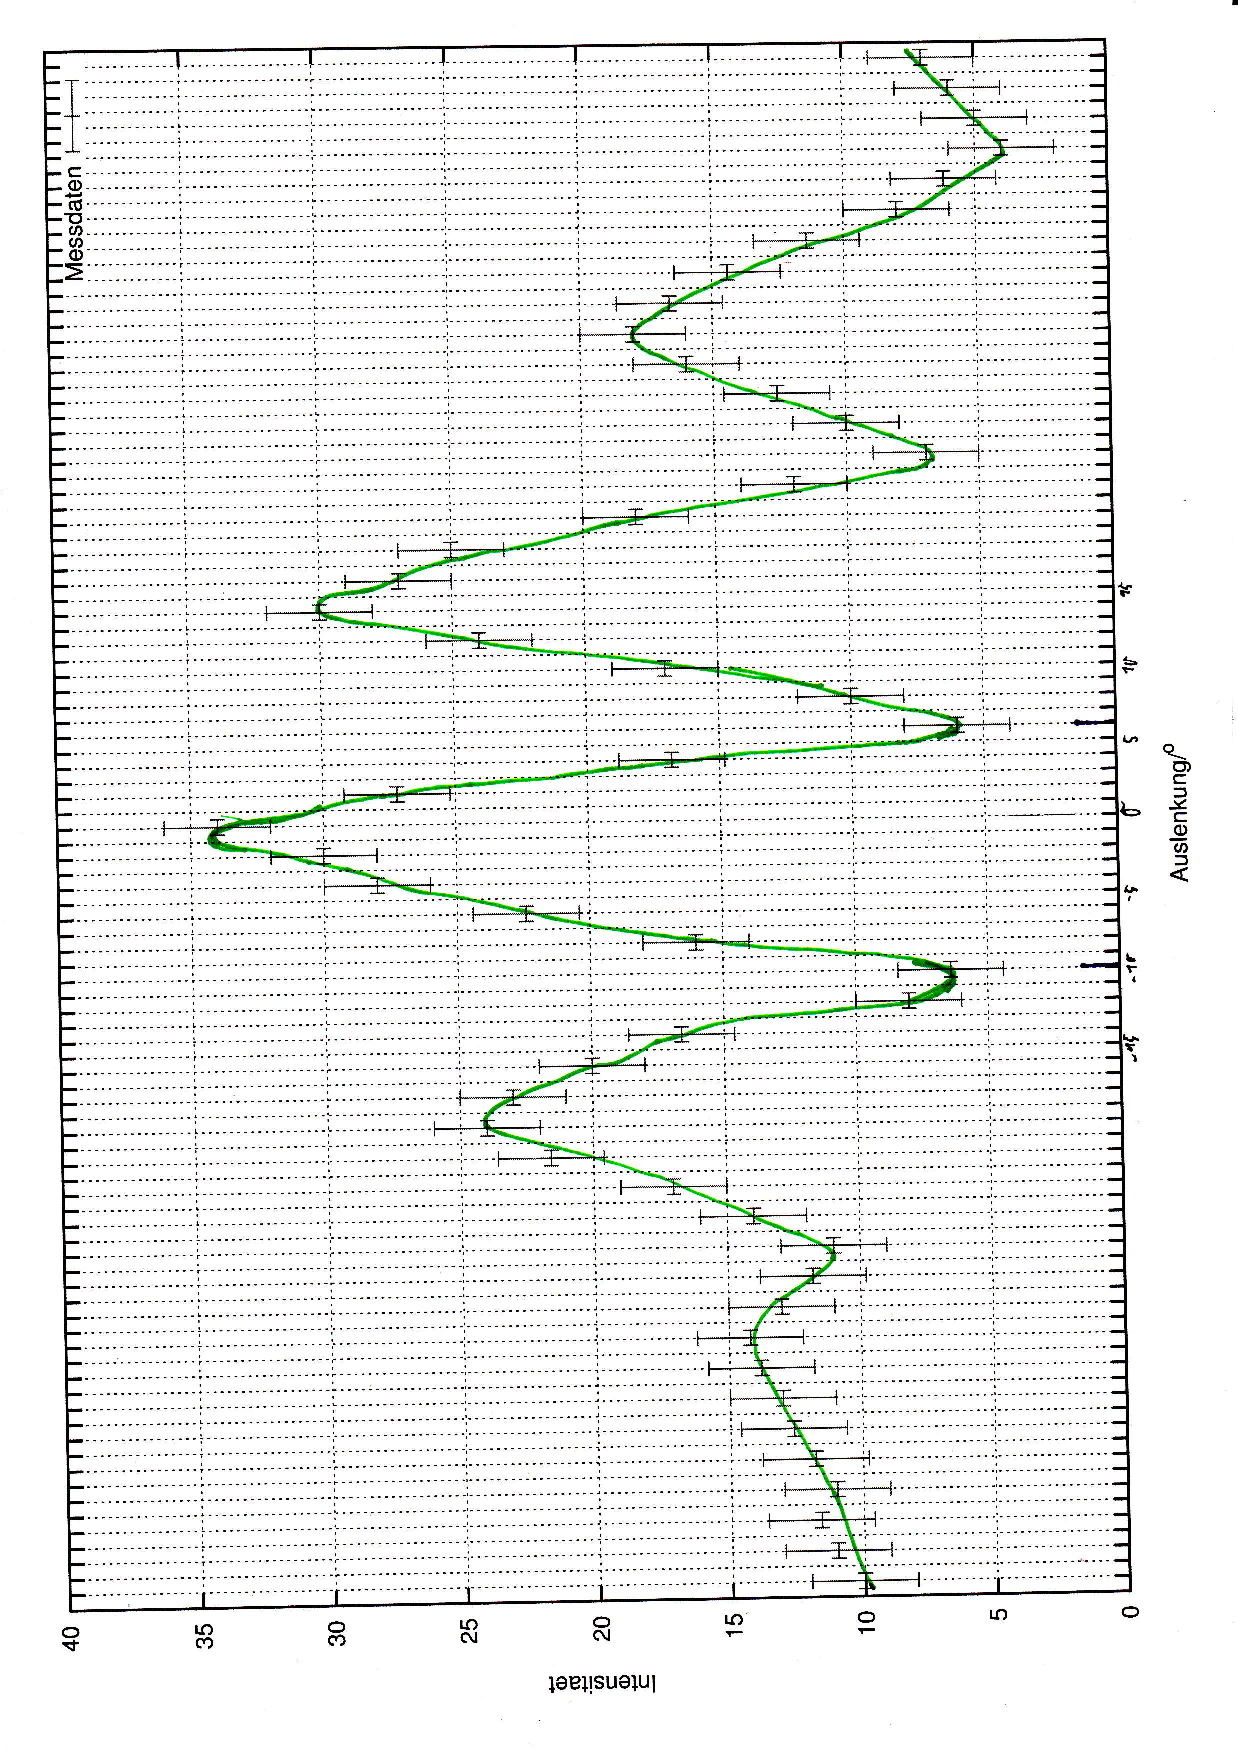
\includegraphics[scale = 0.5, angle = -91]{aufgabe_3_b.pdf}
  	\caption[Plot der Daten aus der Messung zu Aufgabe 3]{Plot der Daten aus der Messung zu Aufgabe 3}
  \label{fig:plot}
\end{figure}
\subsection{Diskussion}
Bei der Messung des Beugungsbildes des Doppelspaltes bzw. Doppelsenders mussten wir feststellen, dass unsere Amplituden während der Messung sehr stark variierten. Dies ist durch andere Ultraschallquellen im Raum erklärbar, da wir unsere Messung parallel zu 3 anderen Gruppen durchgeführt haben. Die Nullage des Aufbaus war nicht feststellbar und verschob sich während wir den Winkel einstellten um etwa 1 Grad, was wir in der Berechnung der Wellenlängen berücksichtigt haben. Insgesamt konnten wir bei dieser Messung deshalb keine guten Messergebnisse erwarten. Mit den beiden in der zweiten Aufgabe berechneten Schallgeschwindigkeiten, und den beiden vom größten Maximum aus gesehenen nächsten Minima, ergeben sich Frequenzen, für die die am Frequenzgenerator eingestellte Frequenz in den ersten zwei Fällen innerhalb des ersten Sigmaintervalls \footnote{mit der Phasengeschwindigkeit $v_{Ph}$} und in den anderen beiden Fällen erst innerhalb des zweiten Sigmaintervalls \footnote{mit der Gruppengeschindigkeit $v_{Gr}$} liegt.

\section{Fazit}
In Aufgabe 1 haben wir bis auf einen Ausreißer die erwarteten Frequenzen gemessen, wobei wir das Minimum bei ca. 320000 Hz nicht finden konnten.\\
Die Schallgeschwindigkeit wurde in Aufgabe zwei mit beiden Methoden recht gut bestimmt, wobei wir mit der Phasenmethode einen genaueren Wert mit einem kleineren Fehler gemessen haben.\\
Ebenso können wir mit der Abstandsmessung per Echolot zufrieden sein, da der genaue Abstand zum Piezoelement nicht genau bekannt war und deshalb abgeschätzt werden musste.
\footnote{An dieser Stelle hätte uns ein systematischer Fehler einen Strich durch die Rechnung machen können.}\\
Die Messung zur Interferenz in Aufgabe 3 war mit Abstand die ungenaueste, da unsere Messwerte sehr stark durch äußere Einflüsse verfälscht wurden. Das Interferenzmuster kann man trotz der starken Schwankungen der Amplitude gut erkennen.\\
Zusammenfassend konnten trotz äußerer Störfaktoren alle drei Messungen so durchgeführt werden, dass unsere Vergleichswerte in den meisten Fällen innerhalb des ersten Sigmaintervalls des Messwertes lagen. 

 %Werte stimmen mit den Formeln überein/nicht überein

\end{document}

